\subsection*{Question 1}
\textbf{Define a randomized detector and a deterministic detector.}

A randomized detector $T$ is $t_{ik} = \textbf{prob}(\hat \theta = i | x = k)$, where, if we observe $x=k$, then the detector returns the hypothesis $\hat \theta = i$ with probability $t_{ik}$. 

A deterministic detector is a detector whose behavior does not involve any randomness, ie. always gives the same result if the same input is processed. So for a deterministic detector, $t_{ik} = 1$ if $\hat \theta = i$ and $0$ otherwise.


\subsection*{Question 2}
\textbf{Define the detection probability matrix.}

The detection probability matrix can be defined as $D = TP$. 

$$
d_{ij} = (TP)_{ij} = \textbf{prob}(\hat \theta = i | \theta = j).
$$

\subsection*{Question 3}
\textbf{Define a convex combination and use it to define a convex set.}

A convex combination of the points $x_1, \dots, x_k \in C$ is a point of the form $\theta_1 x_1 + \cdots+ \theta_k x_k$, with $\theta_1 + \cdots+\theta_k = 1$ and $\theta_i\ge 0$, for all $i = 1,\dots, k$ (ie. a linear combination \( \sum_{i=1}^k \lambda_i x_i \) where each \( \lambda_i \geq 0 \) and \( \sum_{i=1}^k \lambda_i = 1 \)).

A set $C$ is a convex set if and only if it contains every convex combination of its points. (ie. ``every point can be seen by every other point in the set")

\subsection*{Question 4}
\textbf{Make a sketch of a convex set with exactly two corners (this is not in the handouts, think).}

The shaded region in the figure below: 

\begin{figure}[h]
\centering
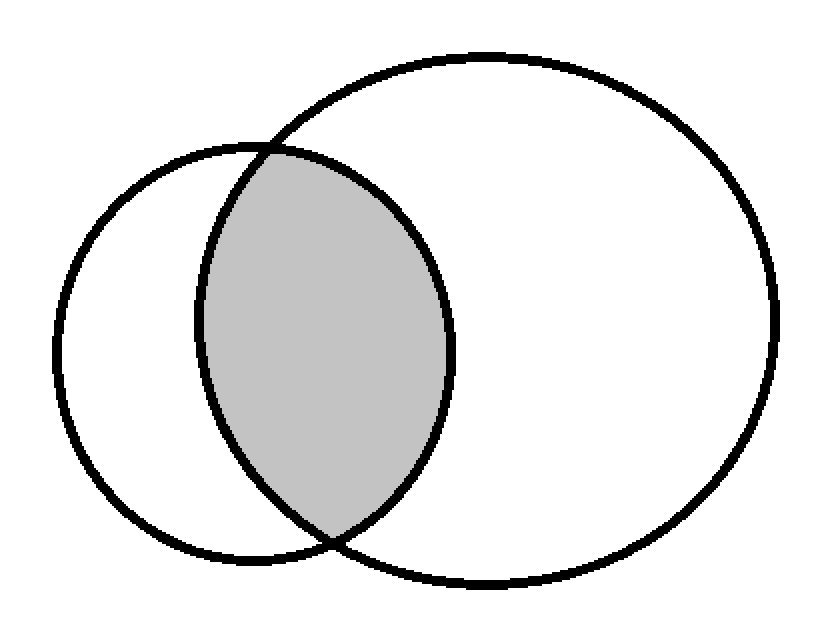
\includegraphics[width=0.5\textwidth]{iRAT/Images/image_2_1.png}
\caption{A convex set with exactly two corners (moon shape)}
\end{figure}

\subsection*{Question 5}
\textbf{Explain the difference between an affine set, a convex set and a conic set.}

An affine set is closed under affine combinations: if every affine combination $\theta_1 x_1 + \cdots+ \theta_k x_k$, with $\theta_1 + \cdots+\theta_k = 1$, of its points  $x_1, \dots, x_k \in C$ belongs to $C$. 

A convex set is closed under concex combinations: it requires that for any \( x, y \in C \) and \( \lambda \in [0,1] \), \( \lambda x + (1-\lambda)y \in C \). This ensures the line segment between any two points is entirely within the set.

A conic set is closed under positive scalar multiplication: for any \( x \in C \) and \( \alpha > 0 \), \( \alpha x \in C \). This makes it a ray of cone region from the origin. 

\subsection*{Question 6}
\textbf{Prove that the positive semidefinite cone is a convex cone using the definition of convex cone (as done in the video of Section 3.3).}

A set \( C \) is a convex cone if for any \( A, B \in C \) and any non-negative scalars \( \alpha, \beta \geq 0 \), the combination \( \alpha A + \beta B \in C \).

Let \( A \) and \( B \) be positive semidefinite matrices, i.e., \( A \succeq 0 \) and \( B \succeq 0 \). Let \( \alpha, \beta \geq 0 \).

Since for any vector \( x \in \mathbb{R}^n \),
\[
x^T (\alpha A + \beta B) x = \alpha x^T A x + \beta x^T B x \geq 0,
\]
givent that \( A \succeq 0 \) and \( B \succeq 0 \).

Therefore \( \alpha A + \beta B \) is positive semidefinite. Hence the positive semidefinite cone is a convex cone.

\subsection*{Question 7}
\textbf{Prove that the positive semidefinite cone is convex using the intersection property (as done in Section 3.4).}

A matrix \( A \in \mathbb{R}^{n \times n} \) is positive semidefinite if and only if for all vectors \( x \in \mathbb{R}^n \), \( x^T A x \geq 0 \).

This condition can be expressed as an intersection of convex sets. For each \( x \in \mathbb{R}^n \), define the set:
\[
C_x = \{ A \in \mathbb{R}^{n \times n} \mid x^T A x \geq 0 \}
\]
Each \( C_x \) is a convex set because it is defined by a linear inequality in terms of \( A \). The positive semidefinite cone \( S_+^n \) is the intersection of all such sets \( C_x \). Since convexity is preserved under intersection, \( S_+^n \) is convex. Hence the positive semidefinite cone is convex.